\chapter{Signal Processing with GPUs}
\label{chap:gpu}

This thesis explores the use of GPUs in data-aided estimation, equalization and filtering operations.
The purpose of chapter is to provide context for the contributions of this thesis.
As such this overview is not a tutorial.
For a full explination of CUDA programming please see the CUDA toolkit documentation \cite{CUDA_toolkit_doc}.

A Graphics Processing Unit (GPU) is a computational unit with a highly-parallel architecture well-suited for executing the same function on many data elements.
In the past, GPUs were used to process graphics data.
Recently, general purpose GPUs are being used for high performance computing in computer vision, deep learning, artificial intelligence and signal processing \cite{wikipedia-gpu:2015}.

GPUs cannot be programmed the way as a CPU. 
NVIDIA released a extension to C, C++ and Fortran called CUDA (Compute Unified Device Architecture).
CUDA allows a programmer to write C++ like functions that are massively parallel called \textit{kernels}.
To invoke parallelism, a GPU kernel is called $N$ times and mapped to $N$ \textit{threads} that run concurrently.
To achieve the full potential of high performance GPUs, kernels must be written with some basic concepts about GPU architecture and memory in mind.

\section{Simple GPU code example}
If a programmer has some C++ experience, learning how to program GPUs using CUDA comes fairly easily.
GPU code still runs top to bottom and memory still has to be allocated.
The only real difference is where the memory physically is and how functions run on GPUs.
To run functions or kernels on GPUs, the memory must be copied from the host (CPU) to the device (GPU).
Once the memory has been copied, the parallel GPU kernels can be called.
After the GPU kernels have finished, the results have to be copied back from the device (GPU) to the host (CPU).

Listing \ref{code:GPUvsCPU} shows a simple program that sums two vectors together where each vector is length $1024$.
\begin{equation}
\begin{matrix}
\mathbf{C}_1 = \mathbf{A}_1 + \mathbf{B}_1 \\
\mathbf{C}_2 = \mathbf{A}_2 + \mathbf{B}_2
\end{matrix}
\end{equation}

On line $42$ the CPU computes $\mathbf{C}_1$ by summing elements of $\mathbf{A}_1$ and $\mathbf{B}_1$ together \textit{sequentially}. Figure \ref{fig:CPUaddBlockDiagram} shows how the CPU computes $\mathbf{C}_1$  sequentially.

The vector addition in the GPU takes a little more work. 
On lines $60$ and $61$ the vectors in host memory $\mathbf{A}_1$ and $\mathbf{B}_1$ are copied to device memory vectors $\mathbf{A}_2$ and $\mathbf{B}_2$.
The vector $\mathbf{C}_2$ is computed by calling the GPU kernel VecAddGPU on line $75$.
The vector is then copied from device memory to host memory on line $78$.
Figure \ref{fig:GPUaddBlockDiagram} shows how the GPU computes $\mathbf{C}_2$ \textit{in parallel}.
\begin{figure}
	\centering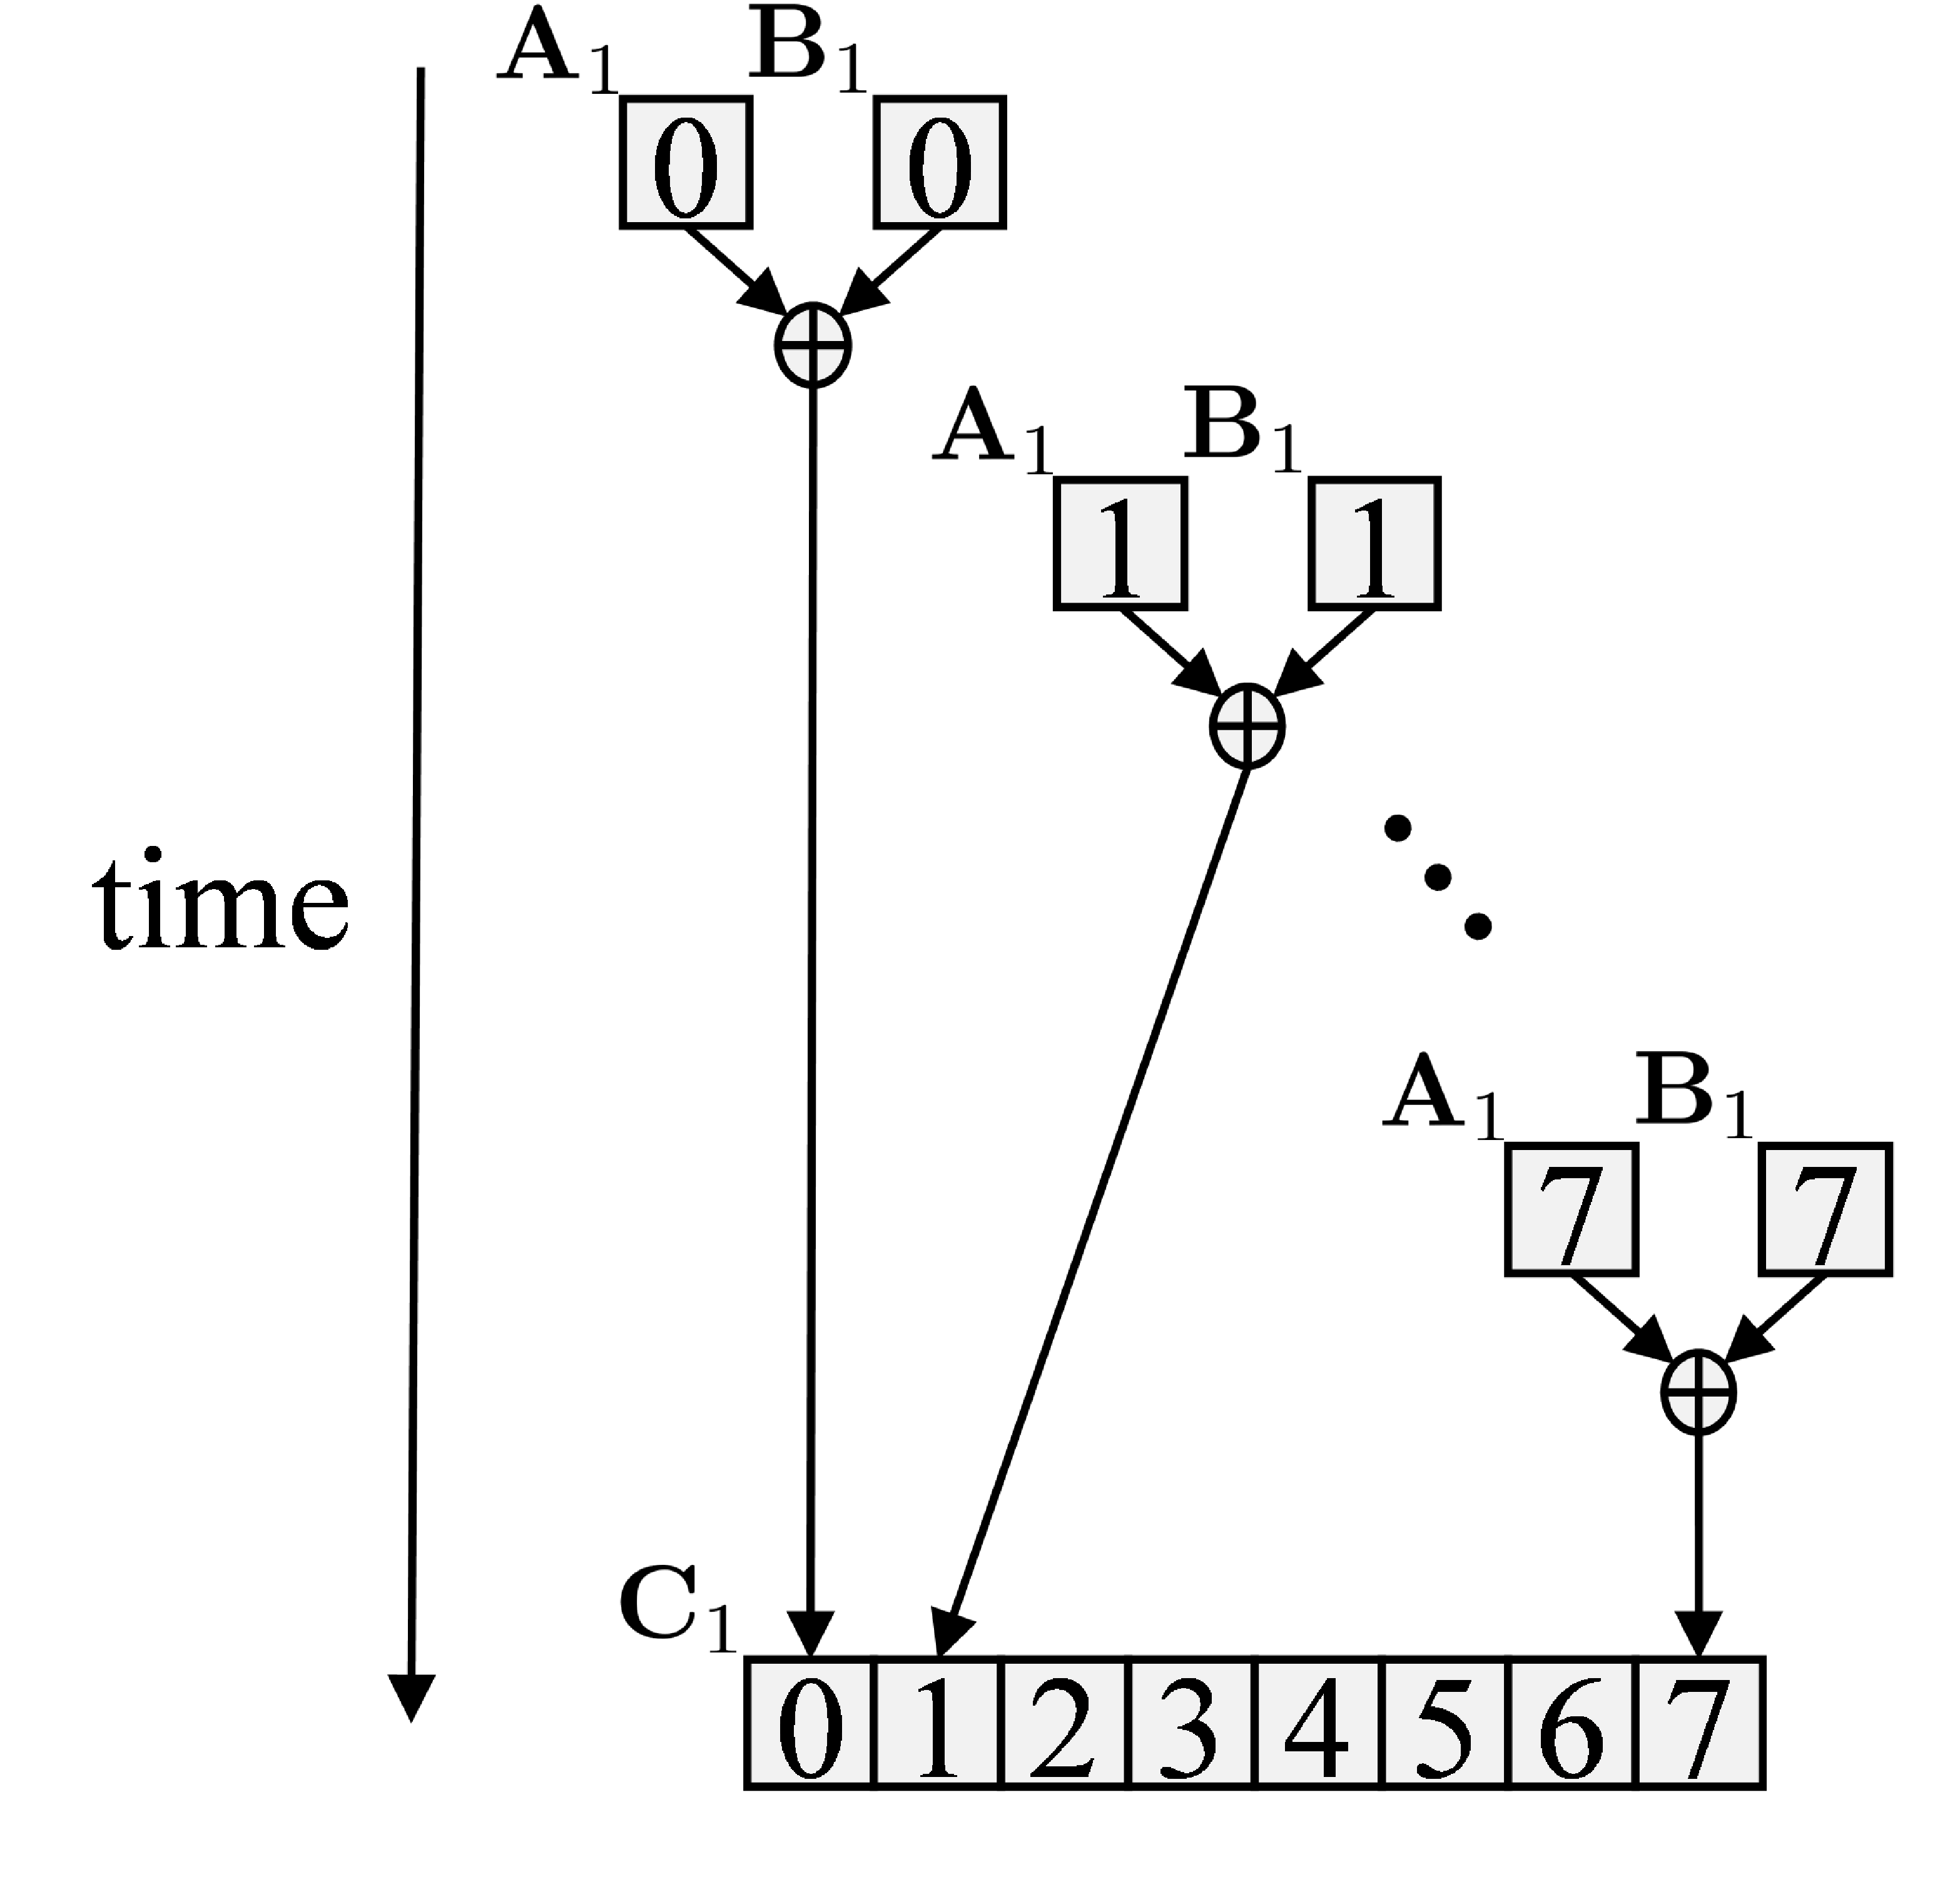
\includegraphics[width=3.17in/100*55]{figures/gpu_intro/CPUaddBlockDiagram.pdf}
	\label{fig:CPUaddBlockDiagram}
	\caption{A block diagram of how a CPU sequentially performs vector addition.}
\end{figure}
\begin{figure}
	\centering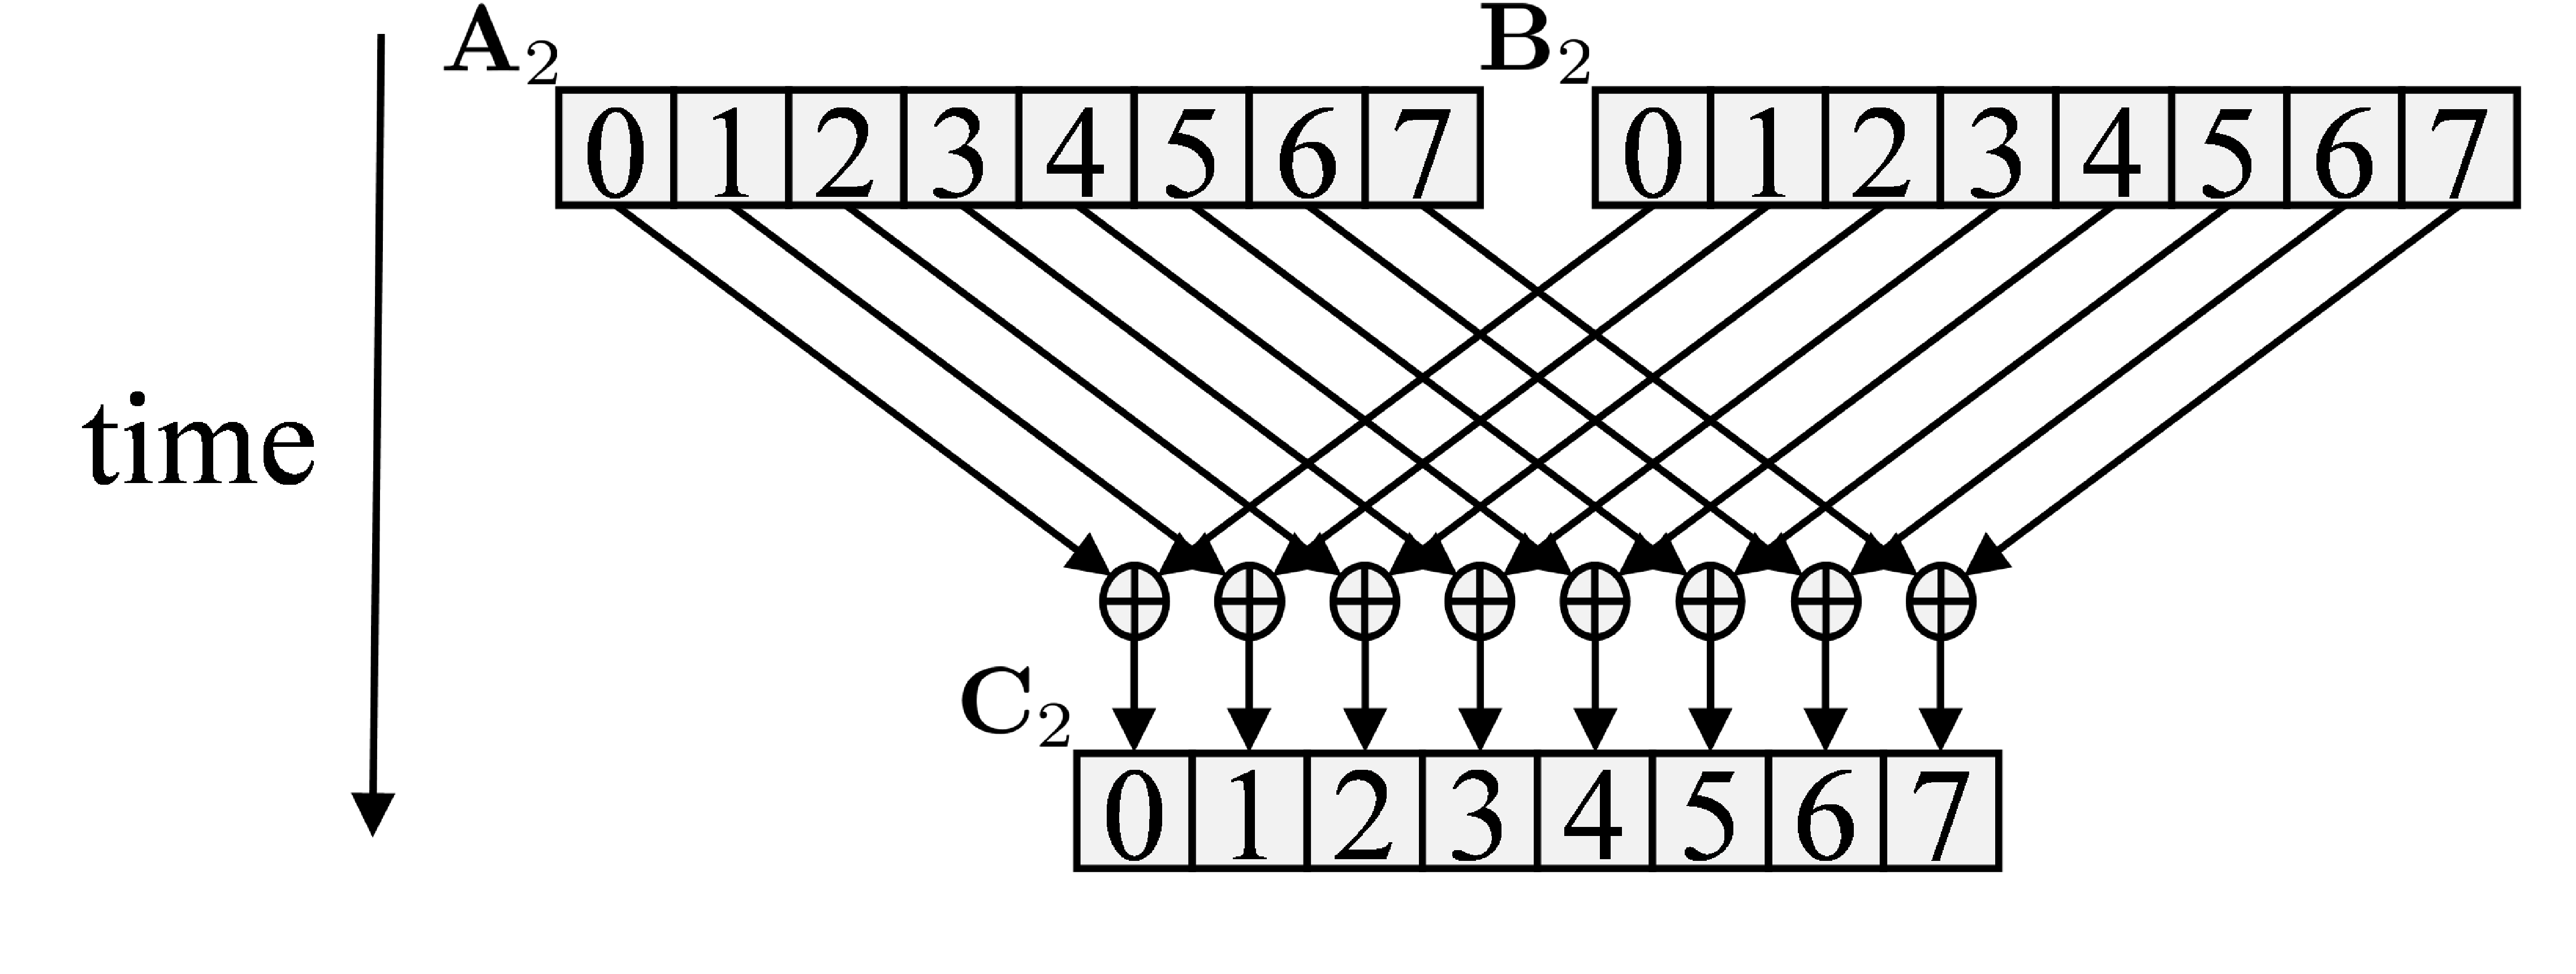
\includegraphics[width=4.69in/100*55]{figures/gpu_intro/GPUaddBlockDiagram.pdf}
	\label{fig:GPUaddBlockDiagram}
	\caption{A block diagram of how a GPU performs vector addition in parallel.}
\end{figure}

\singlespacing
\clearpage
\begin{lstlisting}[style=myCUDAstyle,caption={Comparison of CPU verse GPU code.},label={code:GPUvsCPU}]
#include <iostream>
#include <stdlib.h>
#include <math.h>
using namespace std;

void VecAddCPU(float* destination,float* source0,float* source1,int myLength){
	for(int i = 0; i < myLength; i++)
		destination[i] = source0[i] + source1[i];
}

__global__ void VecAddGPU(float* destination, float* source0, float* source1, int lastThread){
	int i = blockIdx.x*blockDim.x + threadIdx.x;

	// don't access elements out of bounds
	if(i >= lastThread)
		return;

	destination[i] = source0[i] + source1[i];
}

int main(){
	int numPoints = pow(2,22);
	cout << numPoints << endl;
	/**
	* Vector Addition on CPU
	*/
	// allocate memory on host
	float *A1;
	float *B1;
	float *C1;
	A1 = (float*) malloc (numPoints*sizeof(float));
	B1 = (float*) malloc (numPoints*sizeof(float));
	C1 = (float*) malloc (numPoints*sizeof(float));

	// Initialize vectors 0-99
	for(int i = 0; i < numPoints; i++){
		A1[i] = rand()%100;
		B1[i] = rand()%100;
	}

	// vector sum C1 = A1 + B1
	VecAddCPU(C1, A1, B1, numPoints);
	
	/**
	* Vector Addition on GPU
	*/
	// allocate memory on host for result
	float *C2;
	C2 = (float*) malloc (numPoints*sizeof(float));

	// allocate memory on device for computation
	float *A2_gpu;
	float *B2_gpu;
	float *C2_gpu;
	cudaMalloc(&A2_gpu, sizeof(float)*numPoints);
	cudaMalloc(&B2_gpu, sizeof(float)*numPoints);
	cudaMalloc(&C2_gpu, sizeof(float)*numPoints);

	// Copy vectors A and B from host to device
	cudaMemcpy(A2_gpu, A1, sizeof(float)*numPoints, cudaMemcpyHostToDevice);
	cudaMemcpy(B2_gpu, B1, sizeof(float)*numPoints, cudaMemcpyHostToDevice);

	// Set optimal number of threads per block
	int numTreadsPerBlock = 32;

	// Compute number of blocks for set number of threads
	int numBlocks = numPoints/numTreadsPerBlock;

	// If there are left over points, run an extra block
	if(numPoints % numTreadsPerBlock > 0)
		numBlocks++;

	// Run computation on device
	//for(int i = 0; i < 100; i++)
	VecAddGPU<<<numBlocks, numTreadsPerBlock>>>(C2_gpu, A2_gpu, B2_gpu, numPoints);

	// Copy vector C2 from device to host
	cudaMemcpy(C2, C2_gpu, sizeof(float)*numPoints, cudaMemcpyDeviceToHost);

	// Compare C2 to C1
	bool equal = true;
	for(int i = 0; i < numPoints; i++)
		if(C1[i] != C2[i])
			equal = false;
	if(equal)
		cout << "C2 is equal to C1." << endl;
	else
		cout << "C2 is NOT equal to C1." << endl;

	// Free vectors on CPU
	free(A1);
	free(B1);
	free(C1);
	free(C2);

	// Free vectors on GPU
	cudaFree(A2_gpu);
	cudaFree(B2_gpu);
	cudaFree(C2_gpu);
}
\end{lstlisting}
\doublespacing

\section{GPU kernel using threads and thread blocks}
A GPU kernel is executed on a GPU by launching numBlocks thread blocks with a set number of threads per block.
In the Listing \ref{code:GPUvsCPU}, VecAddGPU is launched with $32$ threads per block on line $75$.
The total number of threads launched on the GPU is the number of blocks times the number of threads per block.
VecAddGPU needs to be launched with atleast $2^22$ threads or $131072 = 2^22/32$ blocks of $32$ threads.

CUDA gives each thread launched in a GPU kernel a unique index called threadIdx and blockIdx.
threadIdx is the thread index inside the assigned thread block.
blockIdx is the index of the block that the thread is assigned to.
blockDim is the number of threads assigned per block, in fact blockDim $=$ numTreadsPerBlock.
Both threadIdx and blockIdx are three dimensional and have x, y and z components.
In this thesis only the x dimension is used because GPU kernels operate only on one dimensional vectors.

To turn a CPU for loop in to a GPU kernel that runs $0$ to $N-1$, the GPU kernel will launch atleast $N$ threads are with $T$ threads per thread block.
The number of blocks need is $M = \frac{N}{T}$ or $M = \frac{N}{T}+1$ if $N$ is not an integer multiple of $T$.
Figure \ref{fig:threadsBlocks32} shows $32$ threads launched in $4$ thread blocks with $8$ threads per block.
Figure \ref{fig:threadsBlocks36} shows $36$ threads launched in $5$ thread blocks with $8$ threads per block. 
An full extra thread block is launched with $8$ threads but $4$ threads are idle.
\begin{figure}
	\centering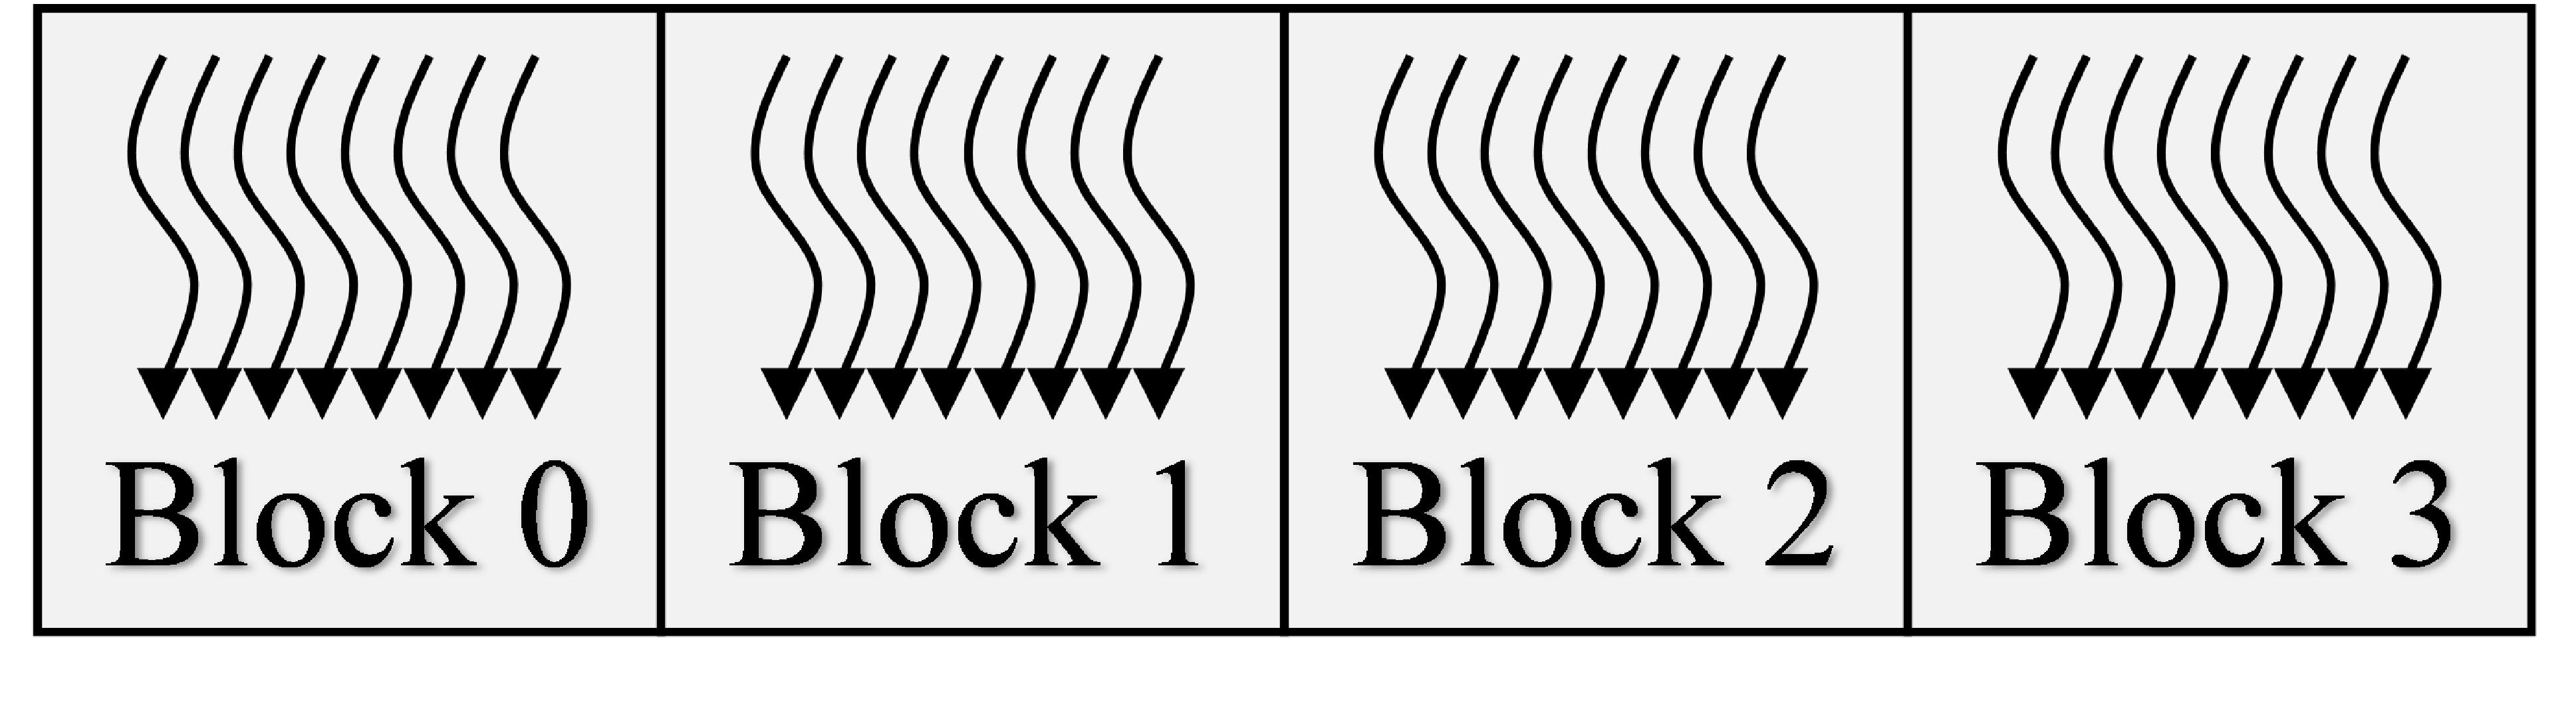
\includegraphics[width=4in/100*55]{figures/gpu_intro/threadsBlocks32.pdf}
	\label{fig:threadsBlocks32}
	\caption{Block $0$ $32$ threads launched in $4$ thread blocks with $8$ threads per block.}
\end{figure}
\begin{figure}
	\centering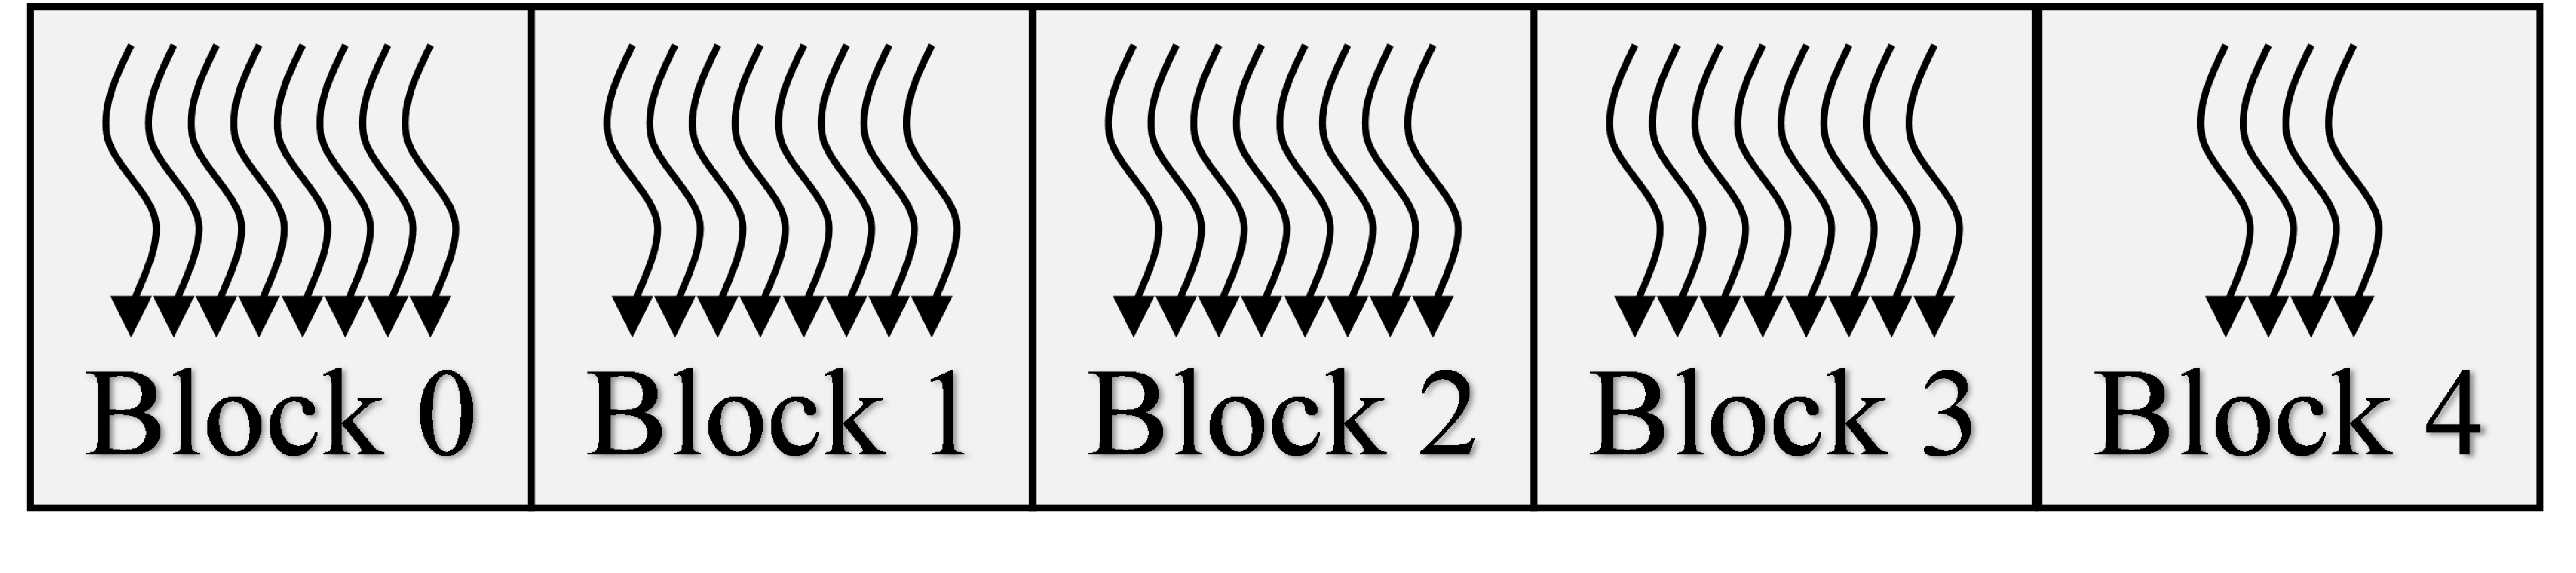
\includegraphics[width=5in/100*55]{figures/gpu_intro/threadsBlocks36.pdf}
	\label{fig:threadsBlocks36}
	\caption{$36$ threads launched in $5$ thread blocks with $8$ threads per block with $4$ idle threads.}
\end{figure}

\section{GPU Execution and Memory}
\label{sec:GPU_memory}
Thread blocks are executed independent of other thread blocks.
The GPU does not guarantee Block $0$ will execute before Block $2$.
Threads in individual blocks can coordinate and use shared memory but blocks do not coordinate with other blocks.
Threads have access to private local memory that is fast and efficient.
Each thread in a thread block has access to shared memory the is private to the thread block.
All threads have access to global memory.

Local memory is the fastest and global memory is by far the slowest.
One global memory access takes 400-800 clock cycles while a local memory in the form of registers, L1 and shared memory is a few clock cycles.
Figure \ref{fig:MemoryPyramid} helps visualize the trade offs of memory and 
Figure \ref{fig:fullGPUmemBlockDiagram} shows where each type of memory is located.
\begin{figure}
	\centering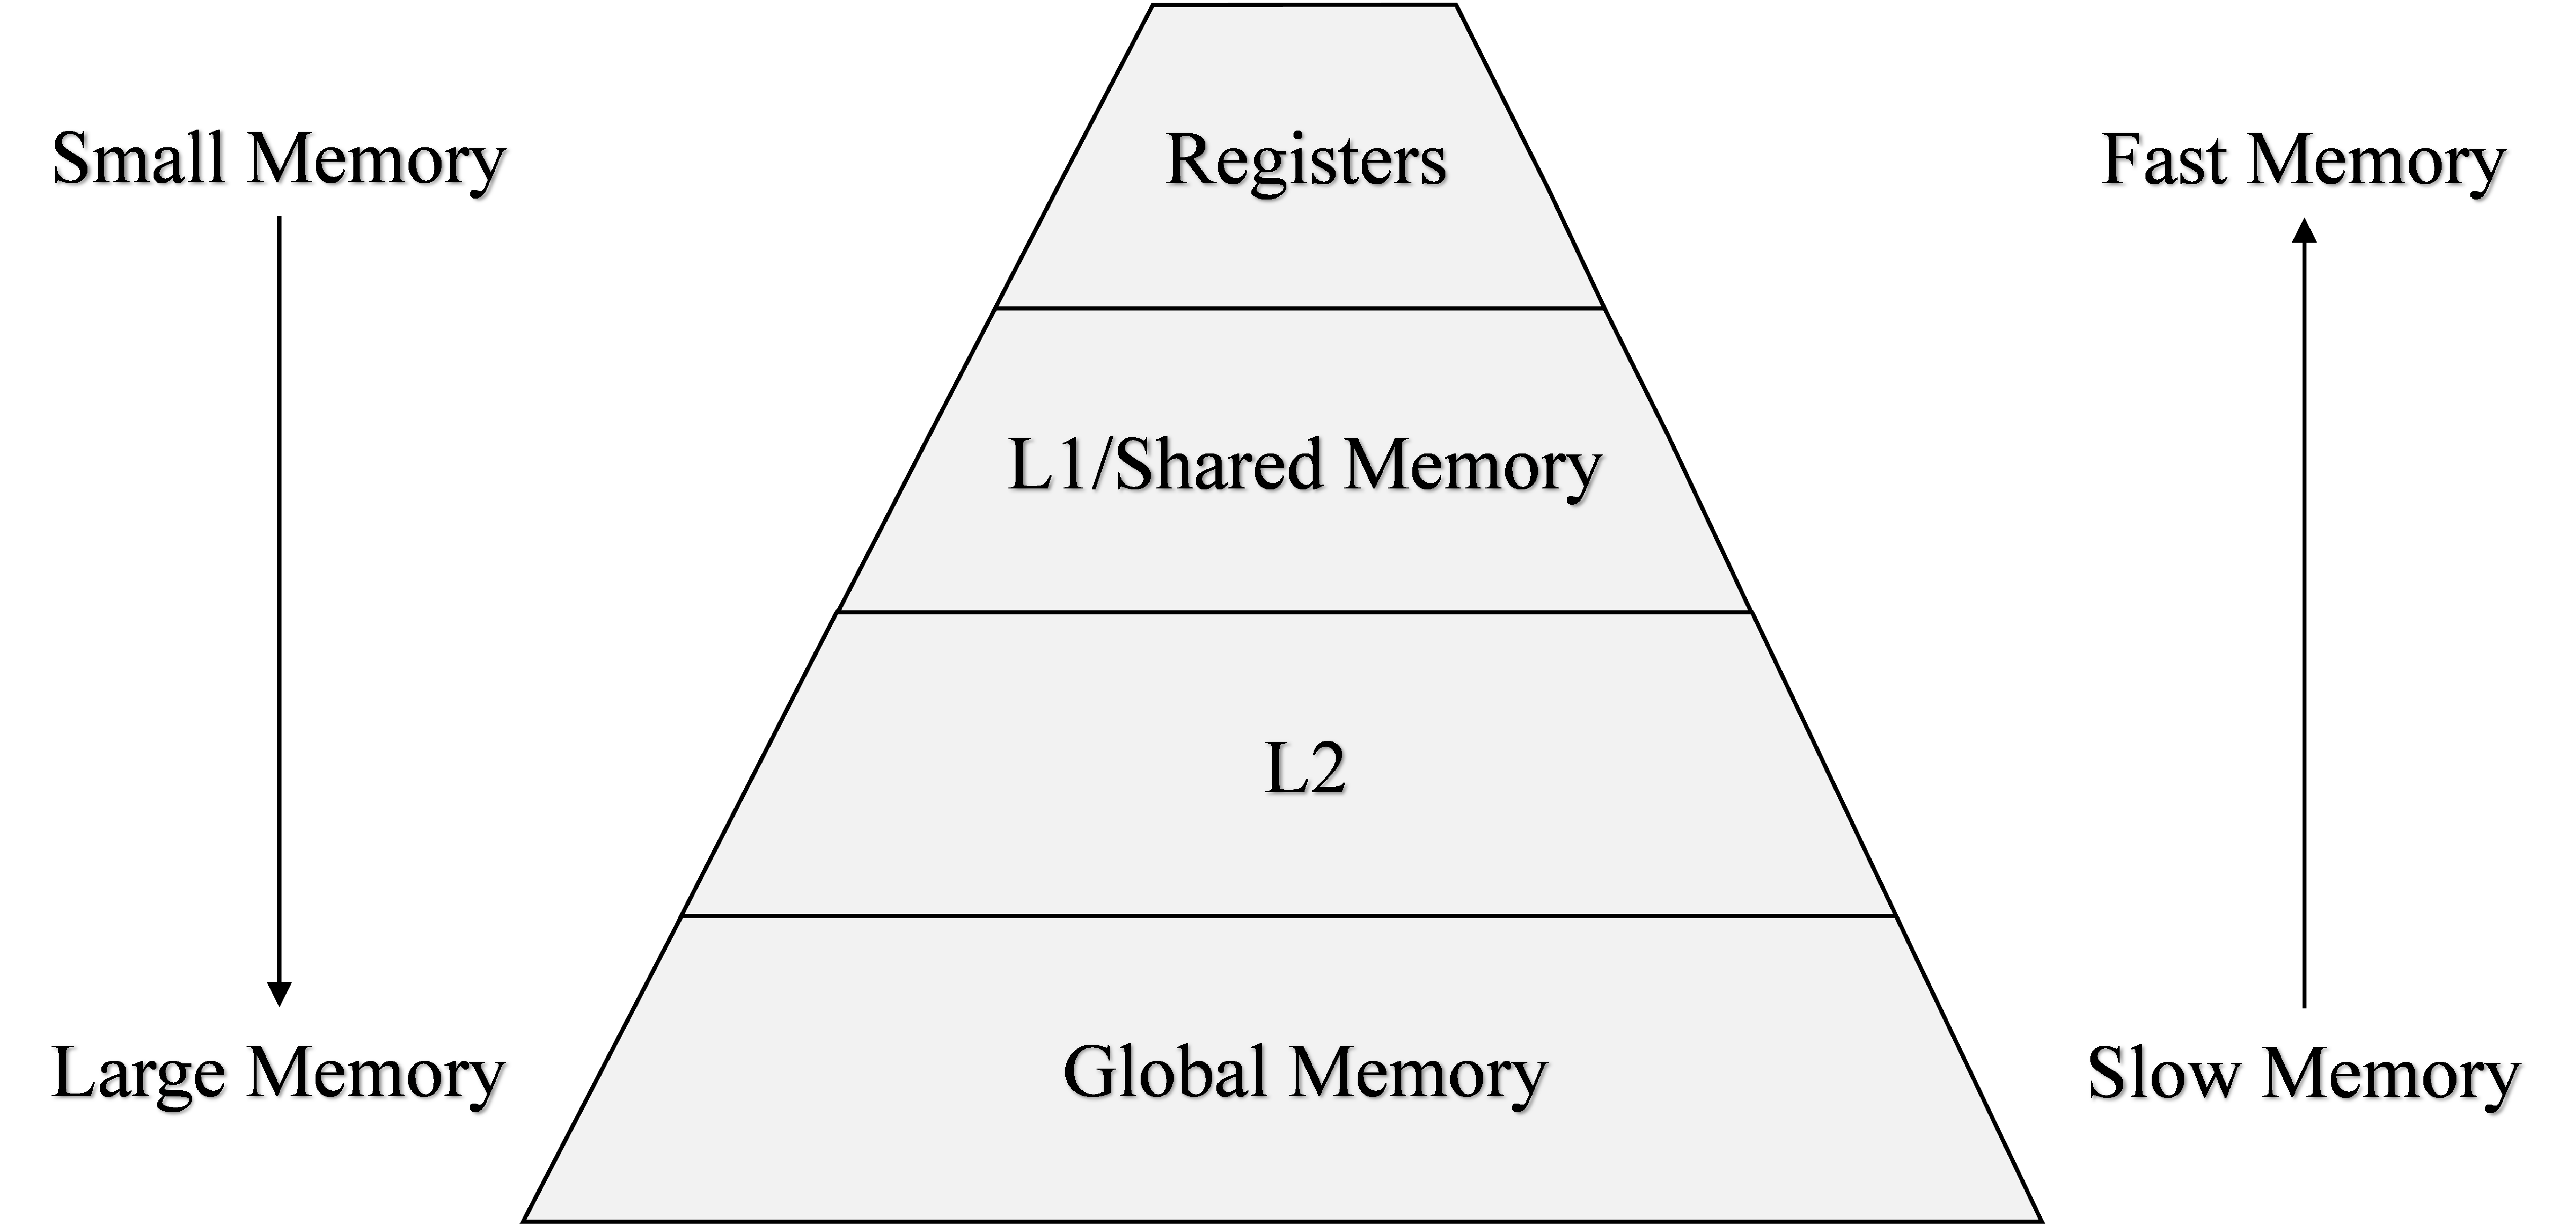
\includegraphics[width=8.36in/100*55]{figures/gpu_intro/MemoryPyramid.pdf}
	\label{fig:MemoryPyramid}
	\caption{Diagram comparing memory size and speed. Global memory is massive but extremely slow. Registers are extremely fast but there are very few.}
\end{figure}
\begin{figure}
	\centering\includegraphics[width=9.83in/100*55]{figures/gpu_intro/fullGPUmemBlockDiagram.pdf}
	\label{fig:fullGPUmemBlockDiagram}
	\caption{A block diagram where local, shared, and global memory is located. Each thread has private local memory. Each thread block has private shared memory. The GPU has global memory that all threads can access.}
\end{figure}

Why not just use local memory for all computation storage?
Elements need to come from global memory to before they can be used in local memory.
If many threads access the same elements in global memory, clock cycles can be saved by copying the elements from global to shared memory.
Local and shared memory should be used as much as possible but sometimes a GPU kernel cant utilized local and shared memory because elements might only be used once.


Why is global memory so slow?
Looking at the physical hardware is instructive.
This thesis uses NVIDIA Tesla K40c and K20c GPUs, Table \ref{tab:gpu-resources_jeffs} lists some specifications and Figure \ref{fig:GPUpicture} shows the form factor of the these GPUs.
The red box in Figure \ref{fig:GPUarch} shows the GPU chip and the yellow boxes show the SRAM that is \textit{off} the GPU chip.

The global memory is located in the SRAM.
To move memory to thread blocks \textit{on} the GPU chip from global memory requires fetching memory from \textit{off} the GPU.
Considering that global memory is off chip, 400-800 clock cycles doesn't sound all that bad.
\begin{figure}
	\centering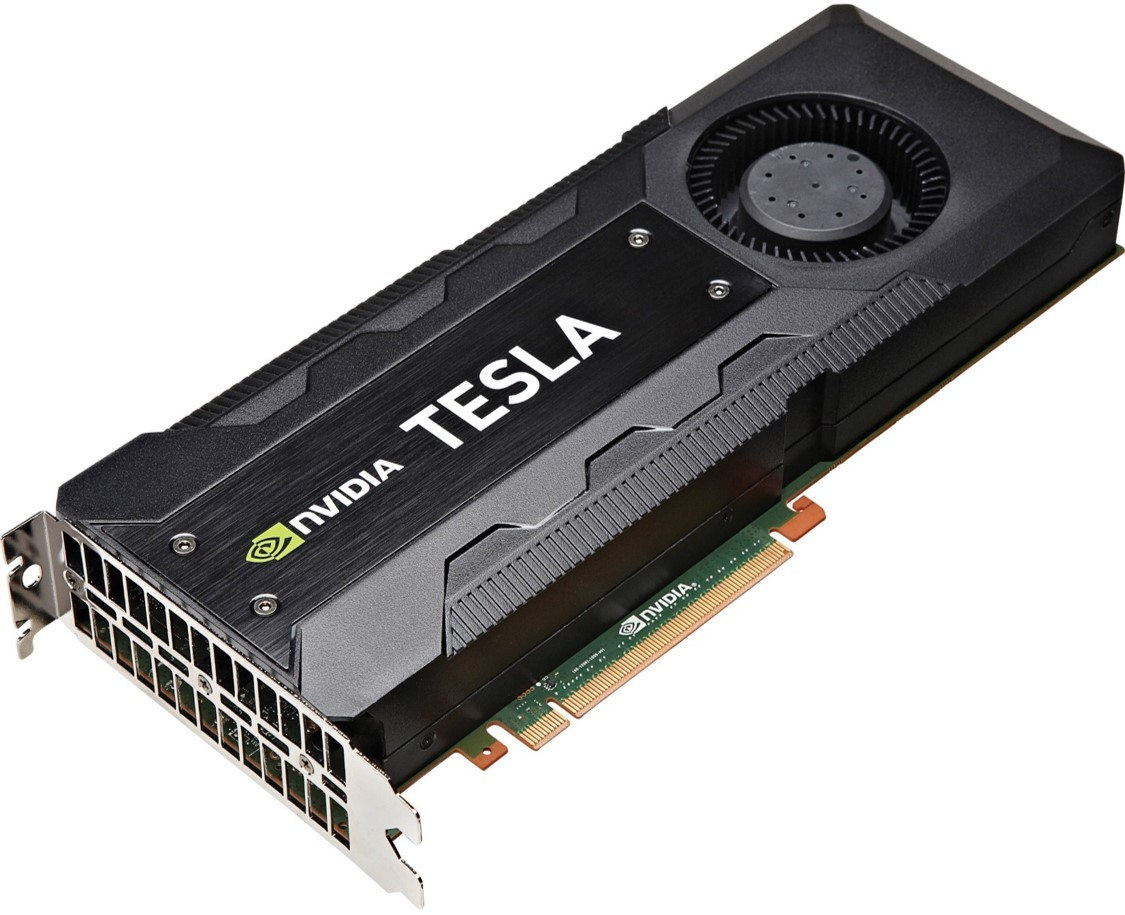
\includegraphics[width=5in]{figures/gpu_intro/k40c_k20c.jpg}
	\label{fig:GPUpicture}
	\caption{NVIDIA Tesla K40c and K20c.}
\end{figure}
\begin{figure}
	\centering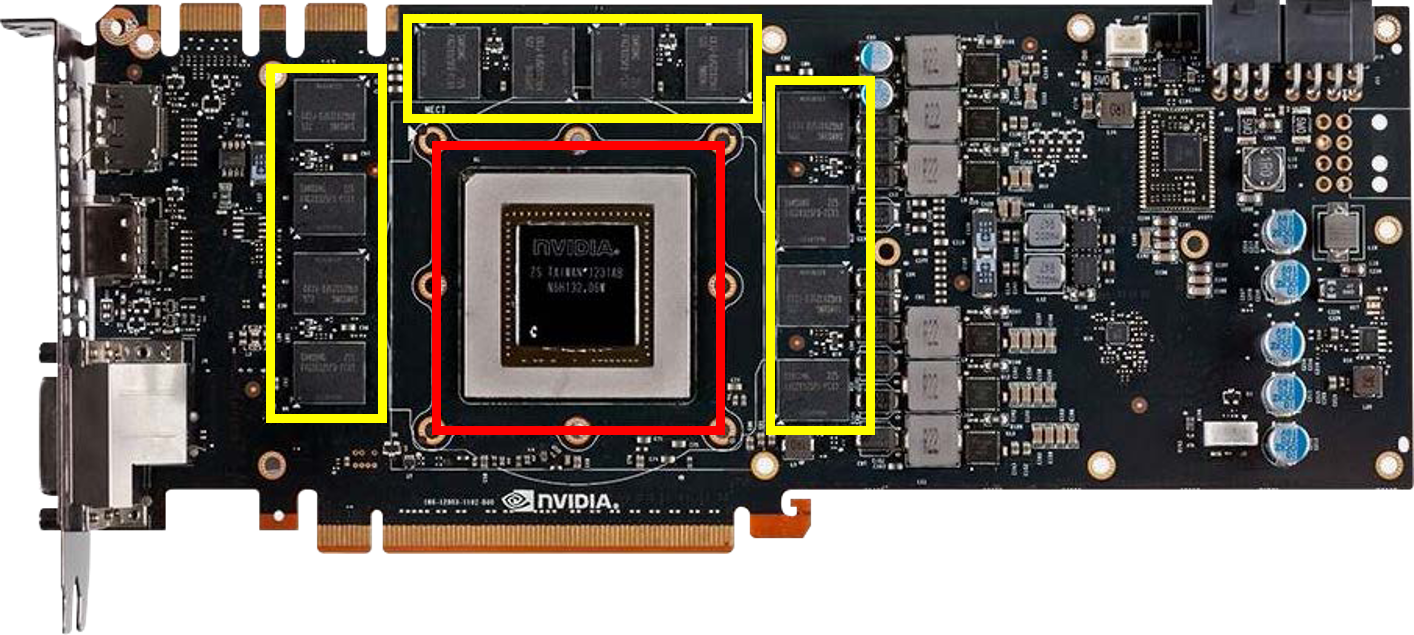
\includegraphics[width=\textwidth]{figures/gpu_intro/Kepler_box.png}
	\label{fig:GPUarch}
	\caption{Example of an NVIDIA GPU card. The SRAM is shown to be boxed in yellow. The GPU chip is shown to be boxed in red.}
\end{figure}
\begin{table}
\begin{center}
\begin{tabular}{lll}
	\toprule
	Feature 			& Tesla K40c 	& Tesla K20c 	\\ \midrule
	Memory size (GDDR5) & 12 GB 		& 5 GB 			\\
	CUDA cores 			& 2880 			& 2496 			\\
	Base clock (MHz) 	& 745 			& 732 			\\ \bottomrule
\end{tabular}
\end{center}
\label{tab:gpu-resources_jeffs}
\caption{The computational resources available with three NVIDIA GPUs used in this thesis (1x Tesla K40c 2x Tesla K20c).}
\end{table}

\section{Thread Optimization}
When writing a custom GPU kernel, it is tempting to launch as many threads per block as possible.
Launching 256 threads per block doesn't sound as fast at launching 1024 threads per block, right?
Wrong. Running the GPU at low occupancy provides each thread with more resources in the each block.
Running the GPU at high occupancy provides each thread with less resources.

Launching 1024 threads per block isnt always bad though.
1024 might be the optimal number of threads per block.
If a GPU kernel was very computationally heavy but didn't require much memory resources, 1024 threads might be a good amount of threads per block.

Improving memory accesses should always be the first optimization when a GPU kernel needs to be faster.
The next step is to find the optimal number of threads per block to launch.
Knowing the perfect number of threads per block to launch is challenging to calculate.
Luckily, there is a finite number of possible threads per block, $1$ to $1024$.
Listing \ref{code:threadTiming} shows a simple test program that times GPU kernel execution time while sweeping the number of possible threads per block.
The number of threads per block with the fastest computation time is the optimal number of threads per block for that specific GPU kernel.

\singlespacing
\clearpage
\begin{lstlisting}[style=myCUDAstyle,caption={Code snippet for thread optimization.},label={code:threadTiming}]
float milliseconds_opt = pow(2,10); // initiaize to "big" number
int numTreadsPerBlock_opt;
int minNumTotalThreads = pow(2,20); // set to minimum number of required threads
for(int numTreadsPerBlock = 1; numTreadsPerBlock<=1024; numTreadsPerBlock++){
	int numBlocks = minNumTotalThreads/numTreadsPerBlock;
	if(minNumTotalThreads % numTreadsPerBlock > 0)
		numBlocks++;
	cudaEvent_t start, stop;
	cudaEventCreate(&start);
	cudaEventCreate(&stop);
	cudaEventRecord(start);
	
	GPUkernel<<<numBlocks, numTreadsPerBlock>>>(dev_vec0, dev_vec1);
	
	cudaEventRecord(stop);
	cudaEventSynchronize(stop);
	float milliseconds = 0;
	cudaEventElapsedTime(&milliseconds, start, stop);
	cudaEventDestroy(start);
	cudaEventDestroy(stop);
	if(milliseconds<milliseconds_opt){
		milliseconds_opt = milliseconds;
		numTreadsPerBlock_opt = numTreadsPerBlock;
	}
}
cout << "Optimal Threads Per Block " << numTreadsPerBlock_opt << endl
cout << "Optimal Execution Time    " << milliseconds_opt      << endl;
\end{lstlisting}
\doublespacing

Most of the time the optimal number of threads per block is a multiple of $32$. 
At the lowest level of architecture, GPUs do computations in \textit{warps}.
Warps are groups of $32$ threads that do every computation together in lock step.
If the number of threads per block is a non multiple of $32$, some threads in a warp will be idle and the GPU will have unused resources.


Figure \ref{fig:ConvGPU_shared_12672_186taps} shows the execution time of an example GPU kernel
The optimal execution time is $0.1078$ms at the optimal $96$ threads per block.
By simply adjusting the number of threads per block, this example kernel can have a $2\times$ speed up.

Adjusting the number of threads per block doesn't always drastically speed up GPU kernels.
Figure \ref{fig:ConvGPU_shared_12672_186taps} shows the execution time for another GPU kernel with varying threads per block.
Launching $560$ does produce about a $1.12\times$ speed up.
\begin{figure}
	\centering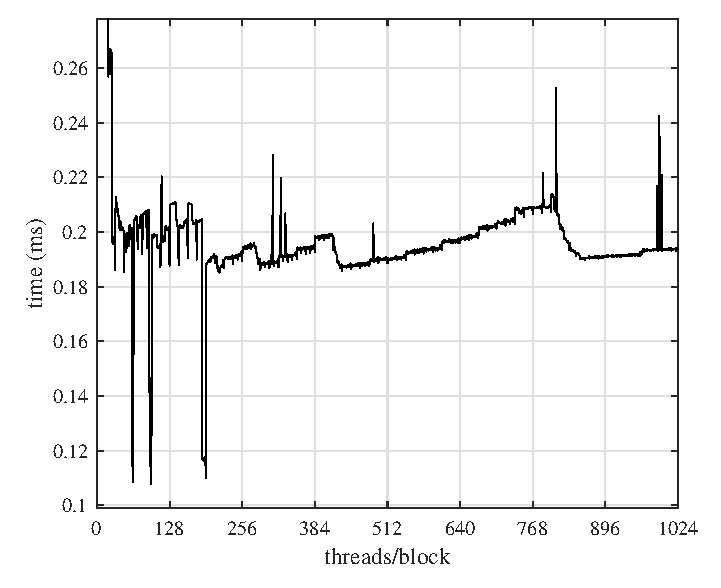
\includegraphics[width=5in]{figures/gpu_intro/ConvGPU_shared_12672_186taps.eps}
	\label{fig:ConvGPU_shared_12672_186taps}
	\caption{Plot showing how execution time is affected by changing the number of threads per block.
	The optimal execution time for an example GPU kernel is $0.1078$ms at the optimal $96$ threads per block.}
\end{figure}
\begin{figure}
	\centering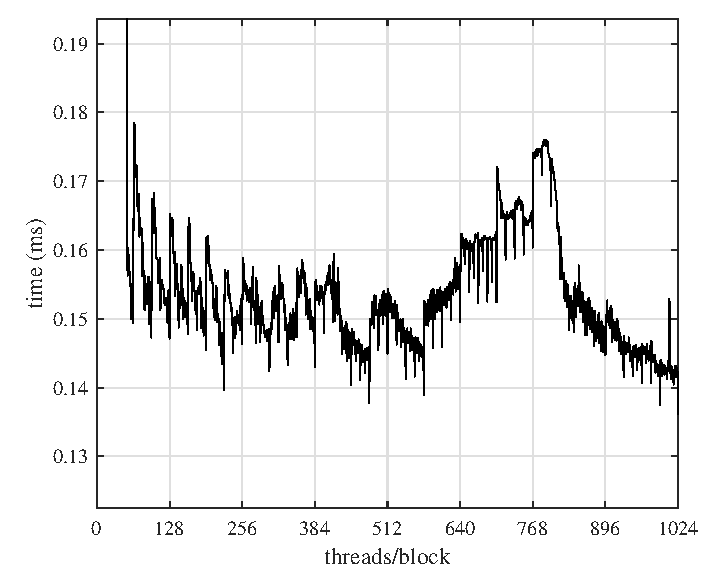
\includegraphics[width=5in]{figures/gpu_intro/ConvGPU_global_12672_186taps.eps}
	\label{fig:ConvGPU_global_12672_186taps}
	\caption{Plot showing the number of threads per block doesn't always drastically affect execution time.}
\end{figure}
%Figure \ref{fig:ConvGPU_shared_12672_186taps} shows the execution time of ConvGPUshared from Listing \ref{code:convFun} while varying threads per block.
%Although the minimum execution time is $0.1078$ms at the optimal $96$ threads per block, but ConvGPUshared must be lauched with atleast $186$ threads per block because of the way the kernel uses shared memory.
%Luckily, launching $192$ threads per block is near optimal with an execution time of $0.1101$ms.
%By simply adjusting the number of threads per block, ConvGPUshared can have a $2\times$ speed up.
%
%Adjusting the number of threads per block doesn't always drastically speed up GPU kernels.
%Figure \ref{fig:ConvGPU_shared_12672_186taps} shows the execution time for ConvGPU with varying threads per block.
%Launching $560$ does produce about a $1.12$x speed up, but thread optimization doesn't have as much of an affect of ConvGPU verse ConvGPUshared.
%\begin{figure}
%	\centering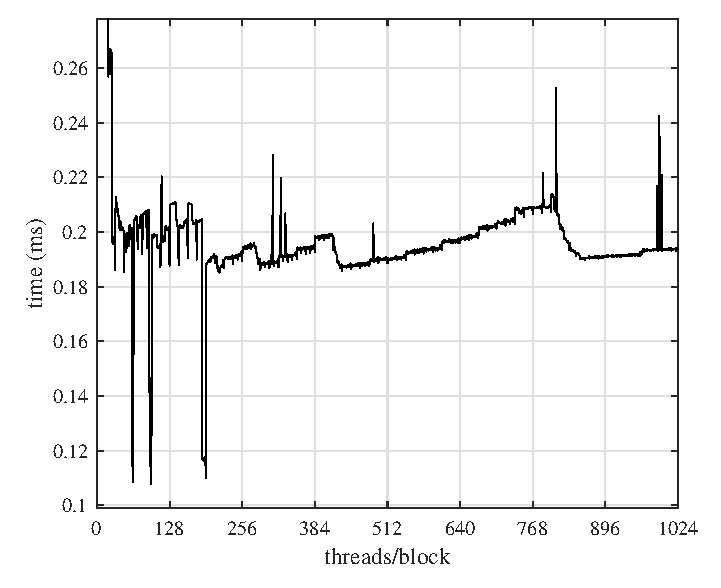
\includegraphics[width=5in]{figures/gpu_intro/ConvGPU_shared_12672_186taps.eps}
%	\label{fig:ConvGPU_shared_12672_186taps}
%	\caption{The GPU convolution thread optimization of a $12672$ length signal with a $186$ tap filter using shared memory. $192$ is the optimal number of threads per block executing in $0.1101$ms. Note that at least $186$ threads per block must be launched to compute correct output.}
%\end{figure}
%\begin{figure}
%	\centering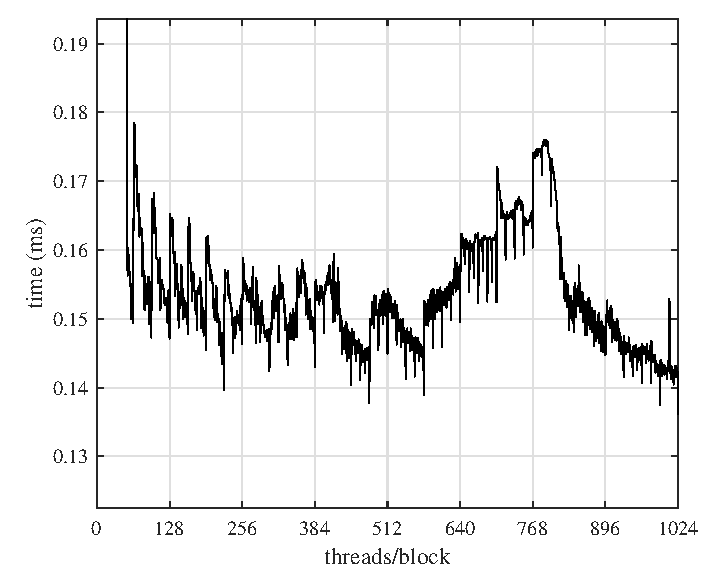
\includegraphics[width=5in]{figures/gpu_intro/ConvGPU_global_12672_186taps.eps}
%	\label{fig:ConvGPU_global_12672_186taps}
%	\caption{ConvGPU thread optimization 128 threads per block 0.006811.}
%\end{figure}
%To answer the question: ``There are $X$ number of ways to implement this algorithm, which one is executes the fastest?'' the answer always is ``It depends. Implement the algorithm $X$ ways and see which is fastest.''

%\section{Cuda Libraries}
While writing a custom GPU kernel then figuring out how to optimize it is extremely satisfying,
CUDA has super optimized GPU libraries that are extremely useful and efficient.
The CUDA libraries are written by NVIDIA engineers that know how to squeeze out every drop of performance out of NVIDIA GPUs.
Some libraries used in this thesis are cuFFT, cuBLAS and cuSolverSp.

\section{CPU GPU Pipelining}
A basic program flow is shown in Listing \ref{code:noPipe}.
The CPU acquires data from myADC on Line 5.
After taking time to acquire data, the data is copied to the CPU, the data is processed in the GPU then result is copied back to the CPU on Lines $8$ to $10$.
cudaDeviceSynchronize on line $13$ causes the CPU to wait until all instructions on the GPU are complete.
Acquiring and copying data takes precious processing time.
What if the GPU could be processing data while the CPU acquires and copied data?
How much computation time could be gained by pipelining acquiring data and processing data?
How much would the throughput increase?

Figure \ref{fig:concurrentCPU_nonBlocking} shows a block diagram of what is happening on the CPU and GPU in Listing \ref{code:noPipe}.
The GPU is idle while the CPU is acquiring data.
The CPU is idle while the GPU is processing and data is being transferred to and from the GPU.
\begin{figure}
	\centering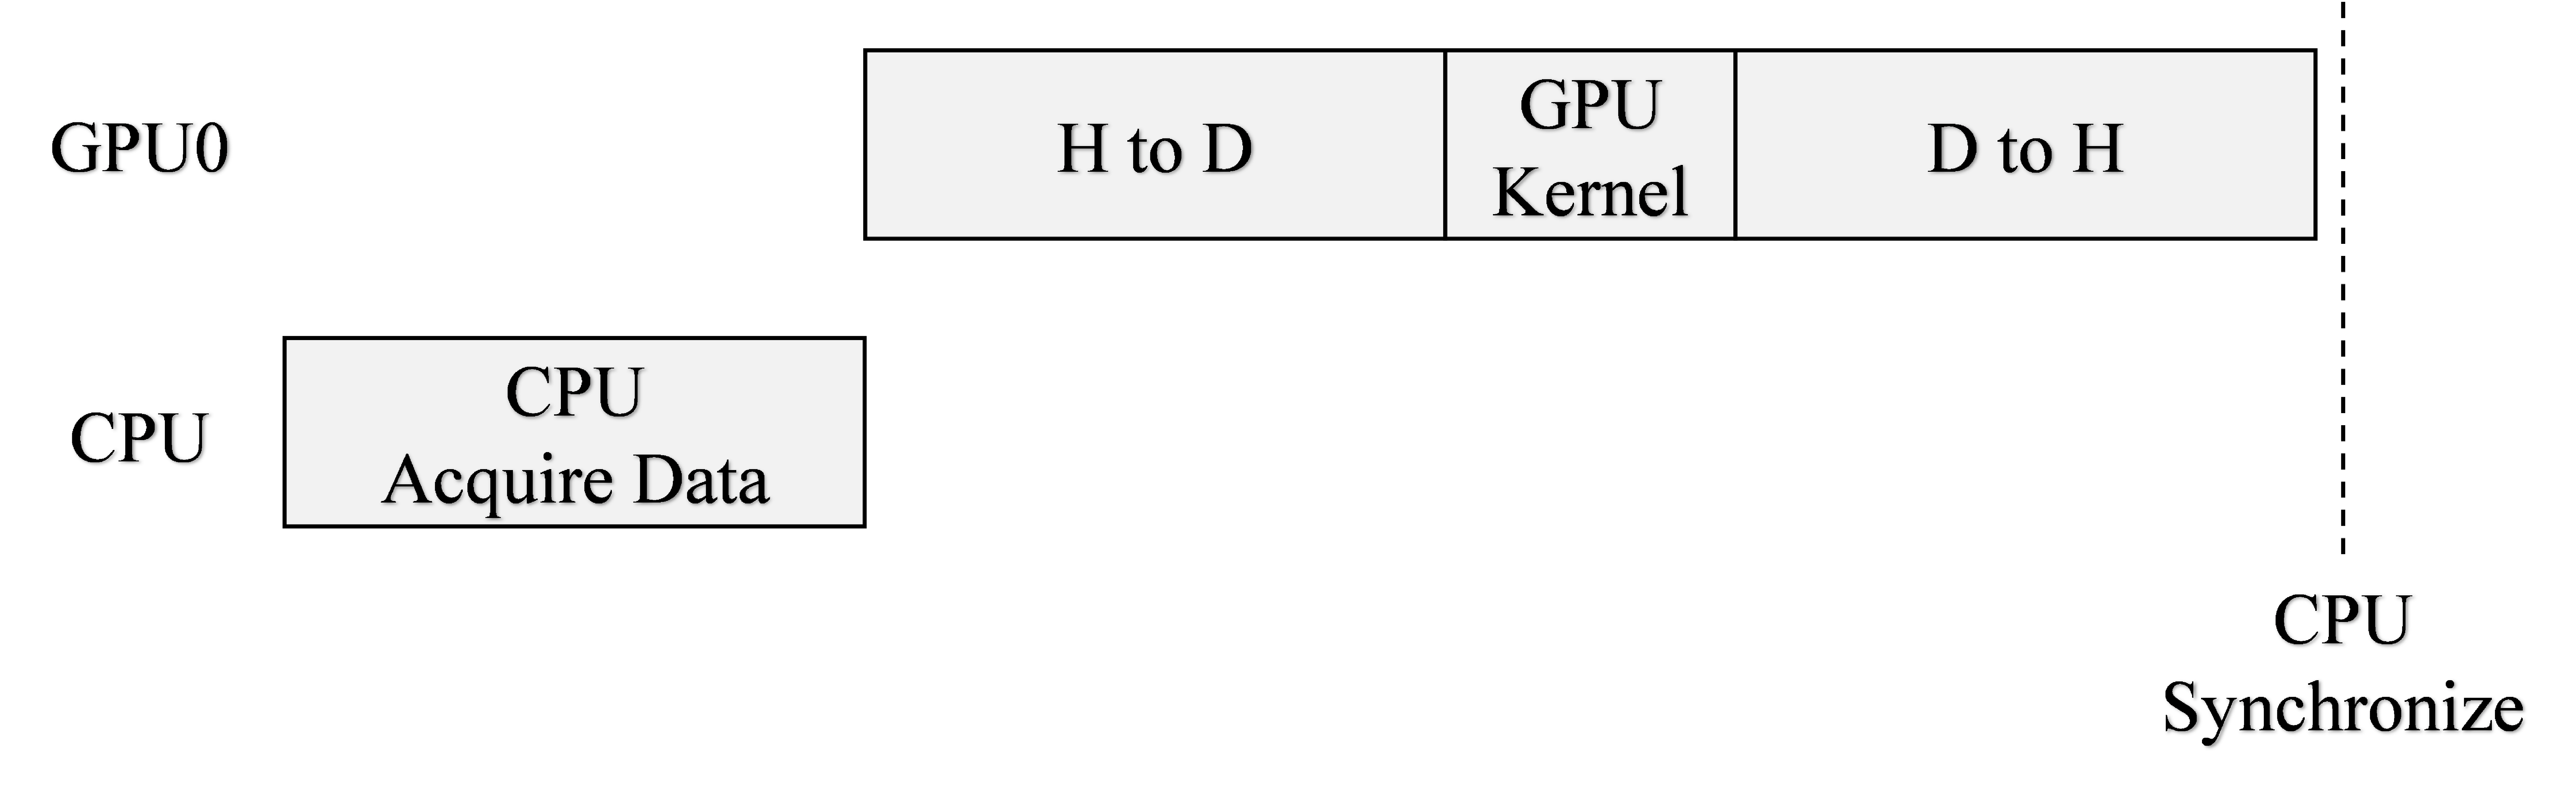
\includegraphics[width=8.77in/100*55]{figures/gpu_intro/concurrentCPU_nonBlocking.pdf}
	\label{fig:concurrentCPU_nonBlocking}
	\caption{The typical approach of CPU and GPU operations. This block diagram shows the profile of Listing \ref{code:noPipe}.}
\end{figure}

\clearpage
\singlespacing
\begin{lstlisting}[style=myCUDAstyle,caption={Example code Simple example of the CPU acquiring data from myADC, copying from host to device, processing data on the device then copying from device to host. No processing occurs on device while CPU is acquiring data.},label={code:noPipe}]
int main()
{
	...
	// CPU Acuire Data
	myADC.acquire(vec);
	
	// Launch instructions on GPU 
	cudaMemcpy(dev_vec0, vec,      numBytes, cudaMemcpyHostToDevice);
	GPUkernel<<<1, N>>>(dev_vec0);
	cudaMemcpy(vec,      dev_vec0, numBytes, cudaMemcpyDeviceToHost);
	
	// Synchronize CPU with GPU
	cudaDeviceSynchronize();
	...
}
\end{lstlisting}
\doublespacing

Can the throughput increase by using idle time on the GPU and CPU?
Yes, CPU and GPU operations can sacrifice latency for throughput by pipelineing.
After the CPU gives instructions to the GPU, the CPU can do other operations like acquire data or perform algorithms better suited for CPUs than the GPUs.
Once the CPU has finished its operations, the CPU can wait for the GPU to finish.

Listing \ref{code:pipe} shows how to pipeline CPU and GPU operations.
Assuming data is already on the GPU from a prior iteration, the CPU gives instructions to the GPU then starts acquiring data.
The CPU then does an asynchronous data transfer to a temporary vector on the GPU.
The GPU first performs a device to device transfer from the temporary vector.
The GPU then runs the GPUkernel and transfers the result to the host.
This system suffers a full cycle latency.
\begin{figure}
	\centering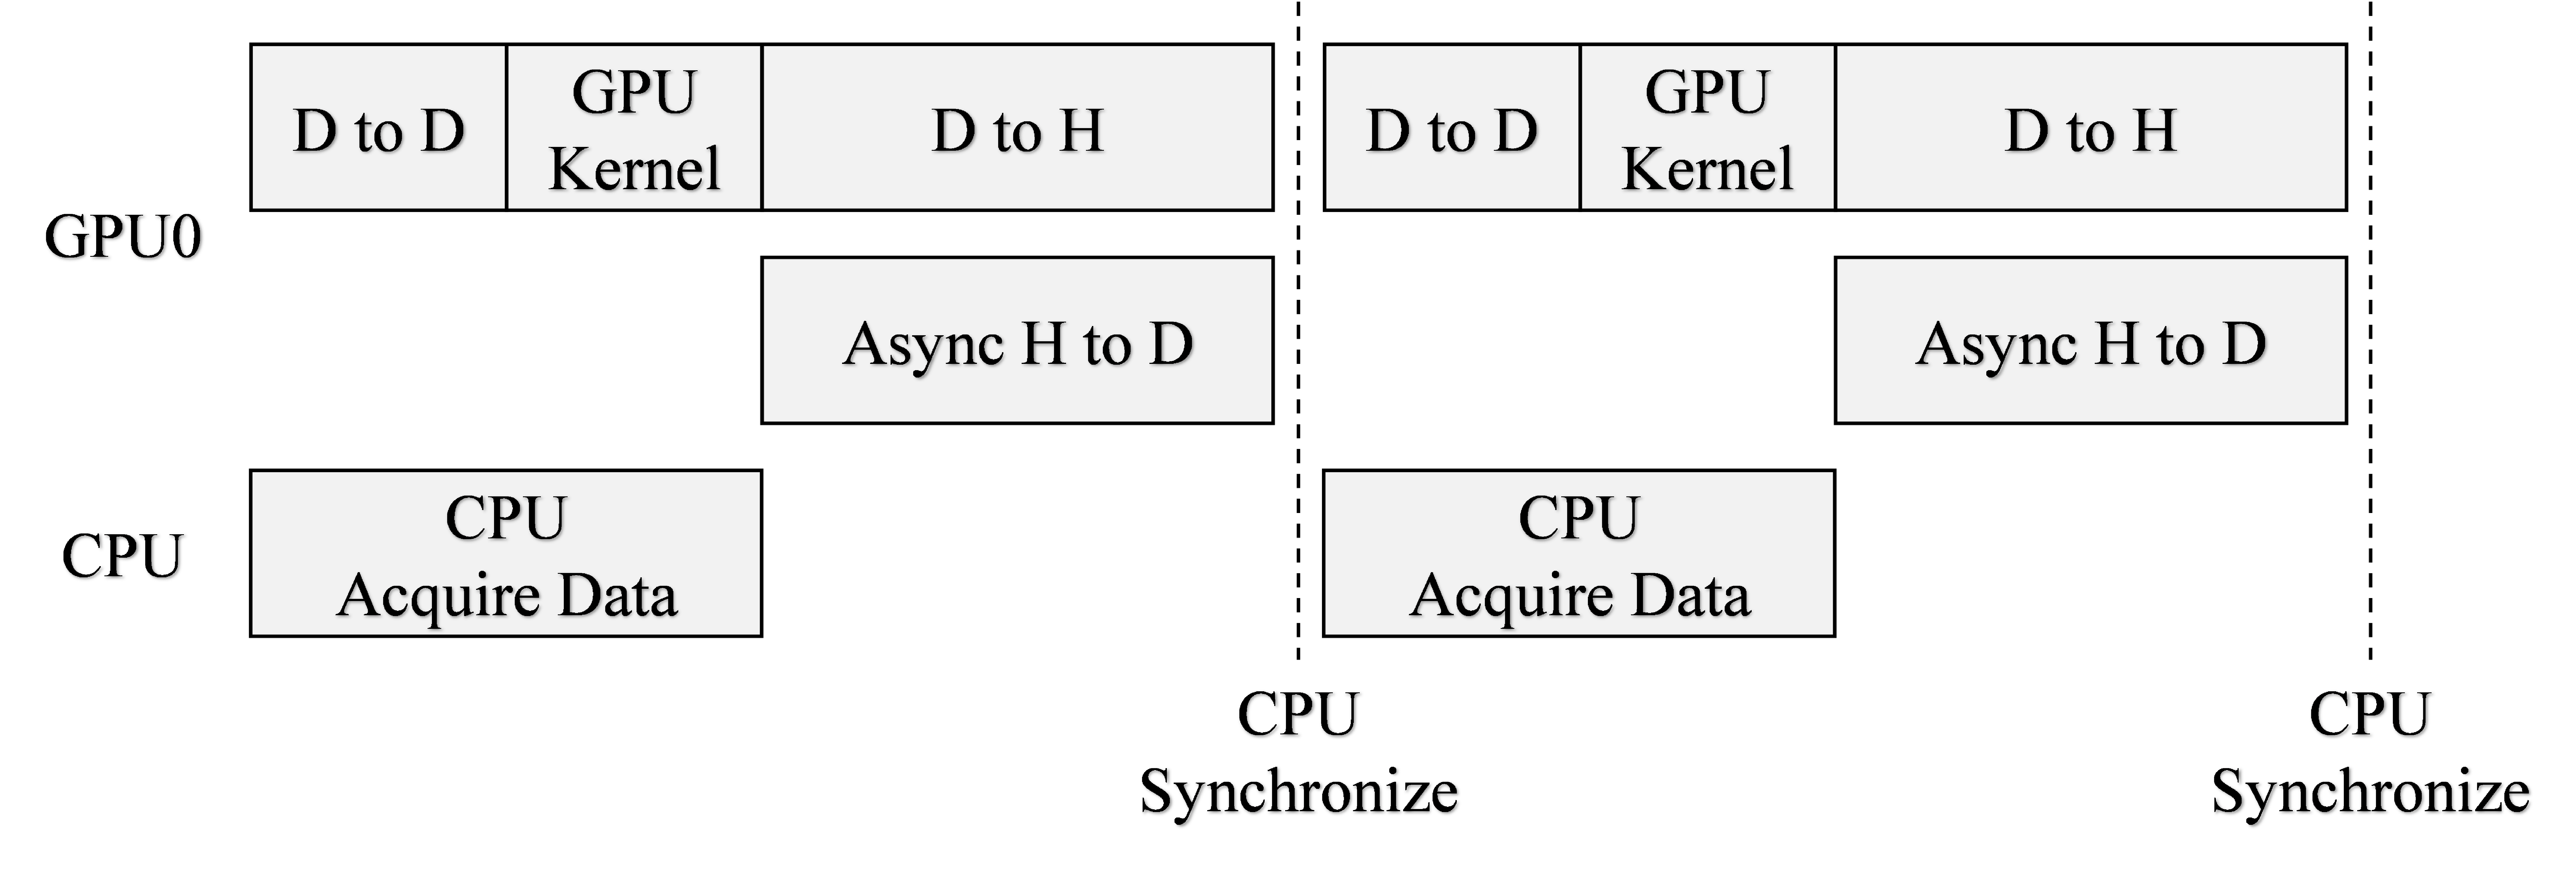
\includegraphics[width=9.97in/100*55]{figures/gpu_intro/concurrentCPU_blocking.pdf}
	\label{fig:concurrentCPU_blocking}
	\caption{GPU and CPU operations can be pipelined. This block diagram shows a Profile of Listing \ref{code:pipe}.}
\end{figure}

\singlespacing
\begin{lstlisting}[style=myCUDAstyle,caption={Example code Simple of the CPU acquiring data from myADC, copying from host to device, processing data on the device then copying from device to host. No processing occurs on device while CPU is acquiring data.},label={code:pipe}]
int main()
{
	...
	// Launch instructions on GPU 
	cudaMemcpy(dev_vec, dev_temp, numBytes, cudaMemcpyDeviceToDevice);
	GPUkernel<<<N, M>>>(dev_vec);
	cudaMemcpy(vec,     dev_vec,  numBytes, cudaMemcpyDeviceToHost);
	
	// CPU Acuire Data
	myADC.acquire(vec);
	cudaMemcpyAsync(dev_temp, vec, numBytes, cudaMemcpyHostToDevice);
	
	// Synchronize CPU with GPU
	cudaDeviceSynchronize();
	...
	
	...
	// Launch instructions on GPU 
	cudaMemcpy(dev_vec, dev_temp, numBytes, cudaMemcpyDeviceToDevice);
	GPUkernel<<<N, M>>>(dev_vec);
	cudaMemcpy(vec,     dev_vec,  numBytes, cudaMemcpyDeviceToHost);
	
	// CPU Acuire Data
	myADC.acquire(vec);
	cudaMemcpyAsync(dev_temp, vec, numBytes, cudaMemcpyHostToDevice);
	
	// Synchronize CPU with GPU
	cudaDeviceSynchronize();
	...
}
\end{lstlisting}
\doublespacing

Pipelineing can be extended to multiple GPUs for even more throughput but only suffer latency of copying memory to one GPU.
Figure \ref{fig:concurrentCPU_nonBlocking_multiGPU} shows a block diagram of how three GPUs can be pipelined.
A strong understanding of the full system is required to pipeline at this level.
\begin{figure}
	\centering\includegraphics[width=11.42in/100*55]{figures/gpu_intro/concurrentCPU_nonBlocking_multiGPU.pdf}
	\label{fig:concurrentCPU_nonBlocking_multiGPU}
	\caption{A block diagram of pipelining a CPU with three GPUs.}
\end{figure}